\documentclass[journal]{IEEEtran}


% correct bad hyphenation here
\hyphenation{op-tical net-works semi-conduc-tor}
\usepackage{amsmath}
\usepackage{comment}
\usepackage{graphicx} 
\usepackage{subfigure}
%\usepackage{cases}
%\usepackage{subeqnarray}

\begin{document}
%
% paper title
% Titles are generally capitalized except for words such as a, an, and, as,
% at, but, by, for, in, nor, of, on, or, the, to and up, which are usually
% not capitalized unless they are the first or last word of the title.
% Linebreaks \\ can be used within to get better formatting as desired.
% Do not put math or special symbols in the title.
\title{Bare Demo of IEEEtran.cls for Journals}
%
%
% author names and IEEE memberships
% note positions of commas and nonbreaking spaces ( ~ ) LaTeX will not break
% a structure at a ~ so this keeps an author's name from being broken across
% two lines.
% use \thanks{} to gain access to the first footnote area
% a separate \thanks must be used for each paragraph as LaTeX2e's \thanks
% was not built to handle multiple paragraphs
%

\author{Michael~Shell,~\IEEEmembership{Member,~IEEE,}
        John~Doe,~\IEEEmembership{Fellow,~OSA,}
        and~Jane~Doe,~\IEEEmembership{Life~Fellow,~IEEE}% <-this % stops a space
\thanks{M. Shell is with the Department
of Electrical and Computer Engineering, Georgia Institute of Technology, Atlanta,
GA, 30332 USA e-mail: (see http://www.michaelshell.org/contact.html).}% <-this % stops a space
\thanks{J. Doe and J. Doe are with Anonymous University.}% <-this % stops a space
\thanks{Manuscript received April 19, 2005; revised September 17, 2014.}}

% The paper headers
\markboth{Journal of \LaTeX\ Class Files,~Vol.~13, No.~9, September~2014}%
{Shell \MakeLowercase{\textit{et al.}}: Bare Demo of IEEEtran.cls for Journals}
% The only time the second header will appear is for the odd numbered pages
% after the title page when using the twoside option.
%
% *** Note that you probably will NOT want to include the author's ***
% *** name in the headers of peer review papers.                   ***
% You can use \ifCLASSOPTIONpeerreview for conditional compilation here if
% you desire.


% make the title area
\maketitle

% As a general rule, do not put math, special symbols or citations
% in the abstract or keywords.
\begin{abstract}
The abstract goes here.
\end{abstract}

% Note that keywords are not normally used for peerreview papers.
\begin{IEEEkeywords}
IEEEtran, journal, \LaTeX, paper, template.
\end{IEEEkeywords}


\IEEEpeerreviewmaketitle



\section{Introduction}
\IEEEPARstart{T}{his}

\section{Related Work}
% lcx
\section{Subsampling and Interpolation}

\subsection{Subsampling}
Resampling using pixel area relation. Suppose $x\times y$ image subsampled down to size $x'\times y'$. scale\_x = x/x', scale\_y = y/y', and then we get block $scale\_x \times scale\_y$, block\_area = $scale\_x \times scale\_y$, the new image's each pixel is the weighted average of pixels in corresponding block's of the original image: 
\begin{align*}
	p'(x',y')=\sum_{i,j}{\frac{covered\_area \cdot p(i,j)}{block\_area}}
\end{align*}
i,j are nonnegative integers, $i \in [scale\_x\times x,scale\_x\times (x+1)]$ $j \in [scale\_y\times y,scale\_y\times (y+1)]$

\subsection{Interpolation}
In the mathematical field of numerical analysis, interpolation is a type of estimation, a method of constructing new data points within the range of a discrete set of known data points. In this project we use bilinear interpolation, bicubic interpolation, Lanczos resampling.

\subsubsection{Bilinear Interpolation}
~\\
\begin{figure}[h]
	\centering
	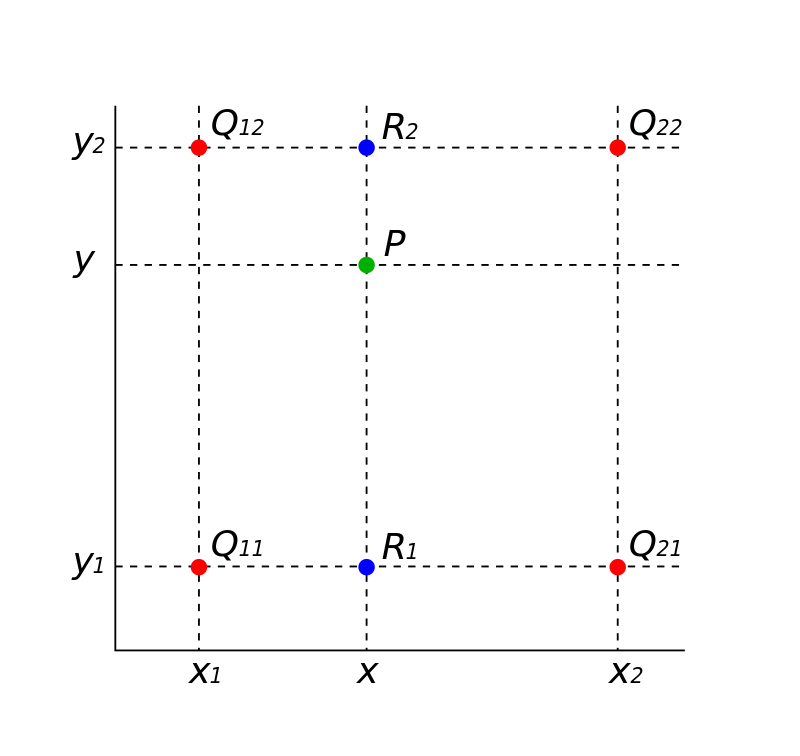
\includegraphics[width=0.6\linewidth]{fig/1.png}
	\label{fig:Bilinear Interpolation}
\end{figure}
\par First do linear interpolation in the x-direction:
\begin{align*}
p(R_1) = \frac{x_2-x}{x_2-x_1}\cdot p(Q_{11})+\frac{x-x_1}{x_2-x_1}\cdot p(Q_{21})\\
p(R_2) = \frac{x_2-x}{x_2-x_1}\cdot p(Q_{12})+\frac{x-x_1}{x_2-x_1}\cdot p(Q_{22})
\end{align*}
Then interpolate in the y-direction:
\begin{align*}
p(P) &= \frac{y2-y}{y2-y1}\cdot p(R_1)+\frac{y-y1}{y2-y1}\cdot p(R_2)\\ &=\small{\frac {1}{(x_{2}-x_{1})(y_{2}-y_{1})}}{\begin{bmatrix}x_{2}-x&x-x_{1}\end{bmatrix}}{\begin{bmatrix}f(Q_{11})&f(Q_{12})\\f(Q_{21})&f(Q_{22})\end{bmatrix}}{\begin{bmatrix}y_{2}-y\\y-y_{1}\end{bmatrix}}
\end{align*}
\par We can get the corresponding pixel's coordinate in original image: $x'\cdot scale\_x=x$, $y'\cdot scale\_y=y$. If either x or y is not integer, $x_1=int(x),x_2=int(x)+1,y_1=int(y), y_2=int(y)+1$, do interpolation.
\par This algorithm reduces some of the visual distortion caused by resizing an image to a non-integral zoom factor.
~\\
\subsubsection{Bicubic Interpolation}
~\\
\par In this method, new image’s pixel at point (x', y'), p(x',y'), is the weighted average of the nearest 16 points in the original image. An interpolator can be obtained by applying a convolution with the following kernel in both dimensions:
\begin{align*}
{\displaystyle W(x)={\begin{cases}(a+2)|x|^{3}-(a+3)|x|^{2}+1&{\text{for }}|x|\leq 1,\\a|x|^{3}-5a|x|^{2}+8a|x|-4a&{\text{for }}1<|x|<2,\\0&{\text{otherwise}},\end{cases}}}
\end{align*}
where a is usually set to −0.5 or −0.75.
\par $x'\cdot scale\_x=x$, $y'\cdot scale\_y=y$. If either x or y is not integer, $x_i$=int(x+i), $y_j$=int(y+j), i, j = -1,0,1,2:

do interpolation in the x-direction:
\begin{align*}
p(x',y_j)=\sum_{i}{W(x-x_i)\cdot p(x_i,y_j)}
\end{align*}
then do interpolation in the y-direction:
\begin{align*}
p(x',y')=\sum_{j}{W(y-y_j)\cdot p(x',y_j)} 
\end{align*}
\par Images resampled with bicubic interpolation are smoother and have fewer interpolation artifacts.
~\\
\subsubsection{Lanczos Resampling}
~\\
\par The effect of each input sample on the interpolated values is defined by the filter's reconstruction kernel L(x), called the Lanczos kernel. 
\begin{align*}
{\displaystyle L(x)={\begin{cases}\operatorname {sinc} (x)\,\operatorname {sinc} (x/a)&{\text{if}}\ -a<x<a,\\0&{\text{otherwise}}.\end{cases}}}
\end{align*}
Equivalently,
\begin{align*}
{\displaystyle L(x)={\begin{cases}1&{\text{if}}\ x=0,\\{\dfrac {a\sin(\pi x)\sin(\pi x/a)}{\pi ^{2}x^{2}}}&{\text{if}}\ -a\leq x<a\ {\text{and}}\ x\neq 0,\\0&{\text{otherwise}}.\end{cases}}}
\end{align*}
\par The parameter $a$ is a positive integer, typically 2 or 3 (but in opencv, the method is cv2.INTER$\_$LANCZOS4, $a$=4), which determines the size of the kernel. The Lanczos kernel has $2a-1$ labes:a positive one at the center, and $a-1$ alternating negative and positive lobes on each side.
\begin{align*}
L(x,y) &= L(x) \cdot L(y)\\
p(x',y') &= \sum_{i,j}{L(x_i-x)\cdot L(y_j-y)\cdot p(x_i,y_j)}
\end{align*}
$x_i=int(x+i)$, $y_j=int(y+j)$, $-a+1\leq i, j \leq a-1$





\section{Conclusion}
The conclusion goes here.






\bibliographystyle{IEEEtran}
\bibliography{Ref}


% that's all folks
\end{document}